\documentclass[12pt, compress]{beamer}
\usepackage{graphicx} %package to manage images
\graphicspath{ {images/} }
\usetheme{m}

\usepackage{booktabs}
\usepackage[scale=2]{ccicons}
\usepackage{minted}


\usemintedstyle{trac}

\title{Introduction to \LaTeX}
\subtitle{Collaboration Tools at UC-Berkeley}
\date{14 February 2017}
\author{Anna Sackmann}
\institute{University of California, Berkeley}

\begin{document}

\maketitle

\begin{frame}[fragile]
  \frametitle{Outline for Today}
    \begin{enumerate}
        \item What is \LaTeX?
        \item Collaboration Tools
        \item Structure of a Document
        \item Basic Commands
        \item A few Exercises
    \end{enumerate}
\end{frame}

\begin{frame}[fragile]
  \frametitle{Introduction}

\LaTeX\ is a typesetting system that allows you to focus on your content instead of formatting - formatting is done separately from entry.
 
 You tell \LaTeX\ ``what it is'' not ``how it looks.''
\end{frame}

\begin{frame}[fragile]
  \frametitle{How Does it Work?}
 {\bf \LaTeX\ vs. \TeX}
  \begin{itemize}
      \item \TeX\ was developed in 1978 as a way for scientists and mathematicians to have better control over their typesetting. \LaTeX came along in the 1980s and takes \TeX to the next level through the use of packages and environments.
      \item Download \LaTeX distribution packages based on their operating systems along with an editor (TeXstudio, TeXmaker, or TeXworks). 
  \end{itemize}
\end{frame}

\section{Collaboration Tools}

\begin{frame}[fragile]
  \frametitle{Share\LaTeX}
  \begin{center}
\includegraphics[scale=0.25]{images/sharelatex.jpg}\end{center}
\end{frame}
  
\begin{frame}{About Share\LaTeX}
    \begin{itemize}
        \item open source 
        \item project history 
        \item smart references and autofill
        \item Dropbox and Github integration 
        \item track changes 
        \item unlimited projects, multiple collaborators per project
    \end{itemize}
\end{frame}

\begin{frame}[fragile]
    \frametitle{Overleaf}
        \begin{center}
\includegraphics[scale=0.5]{images/overleaf.png}\end{center}
\end{frame}
    
\begin{frame}[fragile]
    \frametitle{About Overleaf}
    \begin{itemize}
        \item 10 GB of storage
        \item project history
        \item quick-save to Dropbox
        \item Publisher templates and direct submission process
        \item real-time previews and error-handling
        \item smart references and autofill
    \end{itemize}
\end{frame}

\begin{frame}[fragile]
    \frametitle{Get Your Feet Wet}
    \begin{itemize}
    \item For the most part, type normally.
    \item Words are separated by one or more spaces and paragraphs are separated by one or more lines and are naturally indented. 
    \item Certain symbols require a backslash to appear, like \$ \& \# and \%. 
    \item A \% without a backslash allows you to comment directly in the document.
  \end{itemize}
\end{frame}

\begin{frame}[fragile]
    \frametitle{EXERCISE 1}
        \begin{itemize}
        \item Preambles
        \item Basic Text
        \item Sections
    \end{itemize}
\end{frame}

\begin{frame}[fragile]
    \frametitle{EXERCISE 2}
    \begin{itemize}
        \item Creating Lists
        \item Nesting Lists
    \end{itemize}
\end{frame}

\begin{frame}[fragile]
    \frametitle{EXERCISE 3}
        \begin{itemize}
            \item Exploring Packages in the Preamble
        \end{itemize}
\end{frame}

\begin{frame}[fragile]
    \frametitle{What's Next?}
    Check out Share\LaTeX\ and play around with the interface.
    \begin{itemize}
        \item Is there a tool you prefer?
        \item Why?
    \end{itemize}
    Next, play around with a few different templates. See if you can create a presentation, newsletter, or poster.
\end{frame}

\section{Conclusion}

\begin{frame}[fragile]
    \frametitle{Conclusion}
    \begin{center}A teaser for next week...\end{center}
    \begin{center}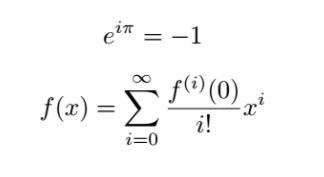
\includegraphics[scale=.5]{images/math.png}\end{center}
\end{frame}

\begin{frame}[fragile]
    \frametitle{Conclusion}
\begin{center}Questions?\end{center}

\begin{center}asackmann@berkeley.edu\end{center}

Check out Typesetting Math in \LaTeX\ on 2.21 

and Creating Tables, Figures, and Bibliographies on 2.28

\end{frame}

\begin{frame}{Summary}

  Get the source of this theme and the demo presentation from

  \begin{center}\url{github.com/matze/mtheme}\end{center}

  The theme \emph{itself} is licensed under a
  \href{http://creativecommons.org/licenses/by-sa/4.0/}{Creative Commons
  Attribution-ShareAlike 4.0 International License}.

  \begin{center}\ccbysa\end{center}

\end{frame}

\end{document}
